\documentclass[UTF8, twoside]{EPURapport}
\usepackage{algpseudocode}
\usepackage{algorithm}
\usepackage{pdfpages}
\usepackage[nottoc, notlof, notlot]{tocbibind}
\usepackage{amsmath,amsfonts,amsthm}
\usepackage{graphicx}
\usepackage{rotating}
\usepackage{color}
\usepackage{colortbl}
%\usepackage{listings}

%\renewcommand{\lstlistlistingname}{Liste des codes}
%\renewcommand{\lstlistingname}{Code}

%\addextratables{%
%	\lstlistoflistings
%}

%\swapAuthorsAndSupervisors



\thedocument{Pattern recognition project draft}{Multi-scale graph comparison}{Multi-scale graph comparison}

\grade{Computer Aided Decision Support\\ International Research Master 2\\ 2013 - 2014}

\authors{%
	\category{Student}{%
		\name{Thomas NOGUER} \mail{thomas.noguer@etu.univ-tours.fr}
	}
	\details{M2RI CADS 2013 - 2014}
}

\supervisors{%
	\category{Supervisors}{%
		\name{Romain RAVEREAUX} \mail{romain.raveaux@univ-tours.fr}
	}
	\details{Université François-Rabelais, Tours}
}

\abstracts{This document presents a method to perform multi-scale graph matching using Louvain's method and the graph edit distance. Results between the classic graph edit distance and this new method are part of this report.}
{Graph matching, community detection, graph edit distance, multi-scale}

\begin{document}

\chapter{Introduction}

	\hspace{4ex}When we wish to do the comparison of two graphs, we can come to a limitation when handling high sized graphs. The community detection algorithms allow to simplify a graph by finding communities of highly related nodes. It is then legitimate to want to use such algorithm to reduce the size of graphs in order to perform calculations that are greedy for computation time.
	
	For this project we chose to use a community detection algorithm for graph comparison. The Louvain's method is very fast and easy to implement. The graph edit distance method is known to be very slow when dealing with high scaled graphs. In this project we want to use the community detection to simplify the graphs to be used in the graph edit distance so we can still compare them with a good computation time.
	
	There is still an issue to solve, how do we use one method with the other. The Louvain's method can be used in several iterations to make the graph more and more simple. We must find a relation between the edit distance of two graphs at different scales and the edit distance between the unchanged graphs. At which scale do we decide that the edit distance is close enough to our original graph? Can we use the different scales together in order to be closer to the distance between the original graphs? These questions are at the center of our problem.
\\

	The rest of the report features the explanation of the graph edit distance and Louvain's method, the elaboration of the multi-scale graph comparison, the results of the project, the perspectives for the future of the project and finally the assessment of this project in regard of my scholarship.
	
\chapter{Graph Edit Distance (GED)}
\label{GED}

	\hspace{4ex}One way to compare two graphs is to use their edit distance. The amount of addition/suppression we must perform to transform a graph G1 into a graph G2. If G1 and G2 are equal their edit distance will be 0, if G1 and G2 are infinitely different from each other their edit distance will be close to infinity.
	
	This method can be very greedy for computation time if the graphs are big, we usually use approach of this value for such graphs. This is what we will try to perform here, find a evaluation of the edit distance that is easier to find.

	We use the following algorithm in order to find the edit distance between two graphs $G1$ and $G2$:
	
\begin{algorithm}
  \caption{Graph Edit Distance}
  \begin{algorithmic}[1]
      \Repeat
      	\For{each node $n \in G1$}
		  \State Add every possible transformation $n$ into the search tree.
		  \State Select a path using $A^*$ and heuristics.
		\EndFor
		\For{each remaining node $n$ of $G2$}
		  \State Add every needed insertion of existing node into the search tree.
		  \State Select a path using $A^*$ and heuristics.
		\EndFor
	  \Until{The path is complete}
	  \State \Return The cost of the found path.
  \end{algorithmic}
\end{algorithm}

\chapter{Community detection: Louvain's method}

	\hspace{4ex}The community detection is used to find communities of highly correlated nodes within a graph. This method is based on two formulas: the modularity $Q$ and the composite modularity gain $\Delta Q$. The modularity of a graph is found following this formula:
\\

\[
Q = \frac{1}{2m}\underset{i,j}{\sum}\left[A_{ij} - \frac{k_ik_j}{2m}\right] \delta(c_i,c_j),
\]

	Where $m$ is the sum of the weights of all the links in the graph ($m = \frac{1}{2}\underset{ij}{\sum}A_{ij}$), $A_{ij}$ the weight of the edge between $i$ and $j$, $k_i$ is the sum of the weights of the edges attached to vertex $i$, $c_i$ is the community to which vertex $i$ is assigned and finally $\delta$ is a function where $\delta(u,v)$ is 1 if $u=v$ and 0 otherwise.
\\
	
	The gain in modularity from moving a node $i$ into a community $C$ is defined by the following formula:
\\

\[
\Delta Q = \left[ \frac{\sum_{in}+k_{i,in}}{2m} - \left( \frac{\sum_{tot}+k_i}{2m} \right)^2 \right] -  \left[ \frac{\sum_{in}}{2m} - \left( \frac{\sum_{tot}}{2m} \right)^2 - \left( \frac{k_i}{2m} \right)^2 \right]
\]

	Where $\sum_{in}$ is the sum of the weights of the links inside the community $C$, $\sum_{tot}$ is the sum of the weights of the links incident to nodes in C and $k_{i,in}$ is the sum of the weights of the links from $i$ to nodes in $C$.
\\

	We use the following algorithm in order to find the communities of our graphs:


\begin{algorithm}
  \caption{Louvain}
  \begin{algorithmic}[1]
      \State Assign each node to a unique community.
      \State Compute the initial modularity.
      \Repeat
      	\For{$i \in V$}
		  \For{$j \in V$}
		  	\State Remove $i$ from its community and place it into $j$'s.
		  	\State Compute the composite modularity gain $\Delta Q$.
		  \EndFor
		  \If{There exists a positive gain}
		  	\State Choose $j$ with the maximum gain and truly move $i$ to $j$'s community.
		  \Else
		  	\State $i$ stays in its community.
		  \EndIf
		\EndFor
	  \Until{No further improvement in modularity}
  \end{algorithmic}
\end{algorithm}

	Our interest in this method here is that it allows us to subdivide our graph into smaller parts that are highly correlated. It will allow us to transform our graphs to make them simpler.

\chapter{Multi-scale graph comparision}

	\hspace{4ex}The main questions remain, how do we use those methods together in order to have a good comparison of graphs? Several approach are possible, do the edit distance at each scale of our graphs and make an average of all the distances. The problem with the majority of the methods we can think about is that they depend on an arbitrary value. What we would like to have is a method that does not depend on a parameter. The method that allow us to do this is to use the classic graph edit distance algorithm on the most simplified graphs by Louvain's method, only that the cost of addition/suppression of a community is equal to its graph edit distance. We have a recursive model that does not depend on the value of a parameter.
	
	\hspace{4ex}We want to compare two graphs G1 and G2. We first use Louvain's method on both graphs until their modularity is not improving, we store the communities of each node at any scale. We then apply the GED algorithm between the most simplified version of both graphs, only when we will evaluate the cost of addition/deletion/substitution of a community (i.e. a node that isn't a node in the original graph G1) we will use the GED of the sub-graph of this community at the previous scale.
	
	In other words, the algorithm will subdivide the calculation of the GED between smaller calculation of GED of parts of our graphs. We hope that this approach will reduce the computation time of the total distance without damaging too much the value of the distance. 
\\

\begin{algorithm}
	\caption{Multi-scale graph edit distance}
	\begin{algorithmic}[1]
		\State // The cost function takes the original graphs and the cost of addition/suppresion for a node and an edge.
		\State Cost $\gets$ CommunityCostFunction(G1, G2, 1, 1)
		\State // G1 is transformed into its simpler version by Louvain's method.
		\State Louvain(G1)
		\State // G2 is transformed into its simpler version by Louvain's method.
		\State Louvain(G1)
		\State // We call the graph edit distance with the simplified version of our graphs and with the special cost function.
		\State \Return GraphEditDistance(G1,G2, Cost)
	\end{algorithmic}
\end{algorithm}

	The community cost function is the following: let us consider two nodes $s$ and $e$, we want to get the cost of addition/suppression of these two nodes only that a node can be a community. We use this cost $GED(GetSubGraph(s),GetSubGraph(e))$ where the function $GetSubGraph(c)$ returns the sub-graph on the community $c$ at the previous scale, or $c$ if $c$ is a node.
	
\chapter{Results}

	\hspace{4ex}In order to see the efficiency of our method we chose to compare it with the classic graph edit distance on a set of small graphs (between 5 to 10 nodes). We performed 9560 comparisons of different graphs with both GED and multi-scale GED.
	
	We can observe in the table \ref{tab:averageResults} that the multi-scale GED is very close to the GED and that its time is far superior in average. From this result we can affirm that the multi-scale GED is a very good estimator of the GED.
	
	The figure \ref{costplot} shows the linear regression of the costs found during the tests. We can notice that the cost of the multi-scale GED is getting closer as the tests progress. It might be because of the size of the graphs that is increasing as the tests progress.
	
	The figure \ref{timeplot} shows the linear regression of the execution times for our two methods. We can spot the huge difference between the execution time of the GED and multi-scale GED.
	
\begin{table}[!h]
\centering
\setlength{\extrarowheight}{1.5pt}
\begin{tabular}{|c|c|c|c|} 
\hline
\multicolumn{2}{|c|}{GED} &  \multicolumn{2}{c|}{Multi-Scale GED}\\
\hline
Cost & Time(ms) & Cost & Time(ms)\\
\hline
1.10 & 324.63 & 2.17 & 8.85\\
\hline
\end{tabular}
\caption{\label{tab:averageResults}Average results for GED and Multi-Scale GED}
\end{table}

\begin{figure} [h]
	\centering 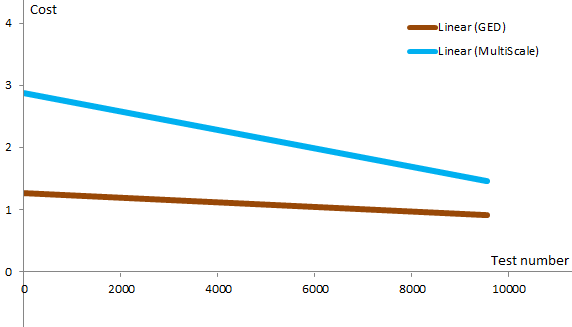
\includegraphics{images/GEDvsMultiScalePlot.png}
	\caption {The linear functions of the costs.}	
	\label {costplot}
\end{figure}

\begin{figure} [h]
	\centering 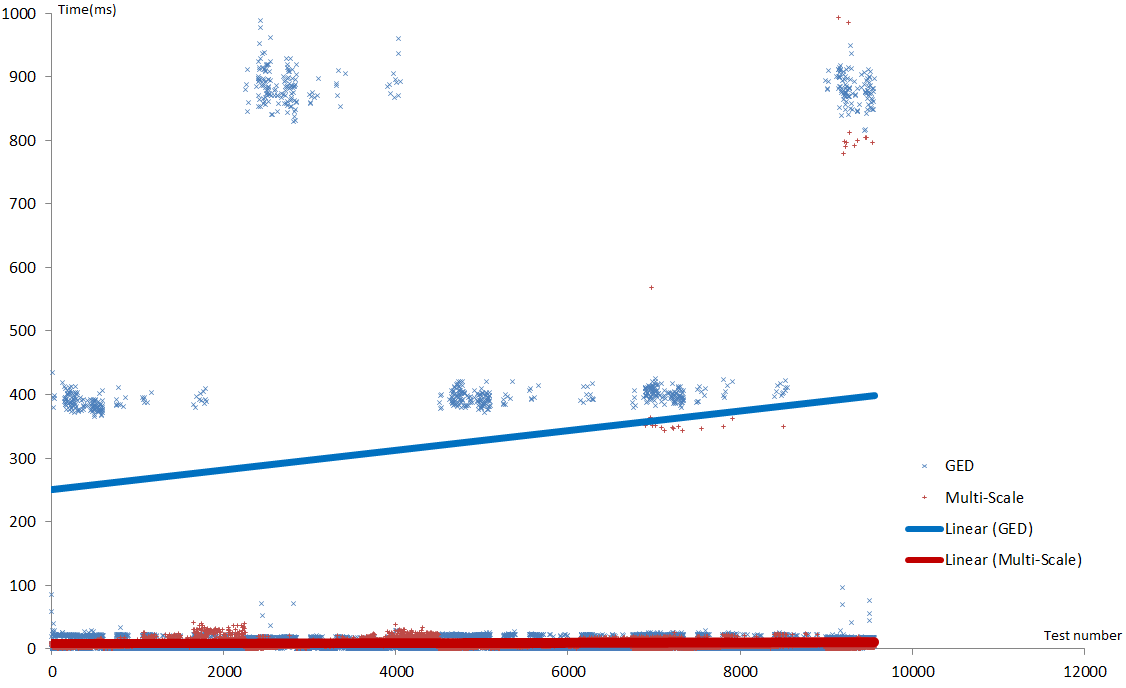
\includegraphics[width=18cm]{images/GEDvsMultiScaleTimePlot.png}
	\caption {The linear functions of the times.}
	\label {timeplot}
\end{figure}

\chapter{Perspectives}

	\hspace{4ex}This project was a first attempt at such a method, much is still to be done. The results are very good and show that the multi-scale graph edit distance is a very good estimator of the edit distance. The most important thing to do is to test this method with graphs of higher size and shapes. Also there seem to still be a bug in the implementation of the method which must be fixed. In a distant future, the method could be used as a upper bound in a branch and bound algorithm or as an approach distance. The project holds publication material that needs to be exploited.

\chapter{Assessment}

	\hspace{4ex}This project was fulfilling as I had never worked on such topics with such methods. The main difficulty has been to master the existing code to be able to add the needed changes. Although this code has been a great help as I had only to implement Louvain's method and adapt the already existing GED, but the recursive approach was not easy to achieve. The given time for this project was short which explains why we have not done further testing on this new method.

\chapter{Conclusion}

	\hspace{4ex}I hope that my work will help further projects and publication, I did my best to make it accessible to future colleges. I would like to conclude by thanking Romain Raveaux for its presence and support during this project.

\begin{thebibliography}{99}	
	
\bibitem{BGLL08}
{\sc Vincent D. Blondel, Jean-Loup Guillaume, Renaud Lambiotte, Etienne Lefebvre}
{\ "Fast unfolding of communities in large networks"}.
{ \textit{Journal of Statistical Mechanics: Theory and Experiment}, 2008}.

\end{thebibliography}

	
\end{document}
